\chapter{\textsc{Clustering of Topics}}
\label{chapter:clustering_of_topics}

This chapter describes the process of clustering the \textit{Topic-grant} and \textit{Topic-researcher} networks. The experiments carried out are detailed, while the results are presented. Additionally, results are evaluated and discussed through comparisons to historical data and between the two Topic networks.

\section{Clustering of Topic-grant network}

The process of clustering the \textit{Topic-grant} network involves a number of different stages including carrying out experiments, producing results, evaluating results as well as conducting comparative analysis.

\subsection{Experiment}

An experiment was carried out in order to identify an optimal edge weight and community detection algorithm. The full settings of the experiment are outlined and detailed in Chapter \ref{chapter:methodology}: Methodology.

The experiment was divided into a number of phases. In the first phase, a number of community detection algorithms were applied to the current \textit{Topic-grant} network constructed using each of the edge weight. The resulting modularity scores of the identified community structure and the number of generated communities were compared across all edge weight and community detection algorithm candidates. Most community detection algorithms make use of the edge weight attribute in the clustering process, which meant that the \textit{unweighted} edge weight had a low performance and was excluded from the experiment in the first phase. Furthermore, a number of community detection algorithms such as \textit{Label Propagation} and \textit{Edge Betweenness} were also excluded due to low performance. In contrast, the \textit{Louvain}, \textit{Spinglass} and \textit{Fast Greedy} algorithms remained to be tested further in the second phase. Table \ref{table:topic_a_current_modularity} presents the results produced during the first phase of the experiment. The edge weights and community detection algorithms considered for the second phase of the experiment are in \textcolor{red}{\textbf{red}}.

\begin{table}[!htbp]
\centering
\caption[Number of communities and modularity score of the community structure identified in the \textit{Topic-grant} network constructed using the current (2010 to 2016) data set]{Number of communities identified (left value) and the modularity score of the community structure discovered (right value) as a result of applying several community detection algorithms to the \textit{Topic-grant} network constructed using the current (2010 to 2016) data set. Three of the column names are abbreviated: \textbf{uw}, \textbf{wnn} and \textbf{wnv} stand for unweighted, weighted by normalized number of grants and weighted by normalized value of grants, respectively. High-performance candidates are in \textbf{\textcolor{red}{red}}.}
\label{table:topic_a_current_modularity}
\begin{tabular}{r|rrrrrr}
\textbf{} & \multicolumn{2}{c}{\textbf{uw}} & \multicolumn{2}{c}{\textcolor{red}{\textbf{wnn}}} & \multicolumn{2}{c}{\textcolor{red}{\textbf{wnv}}}\\
\hline\\
\textbf{Infomap}             & {3}   & {0.004} & {9}   & {0.332} & {11}  & {0.377}\\
\textcolor{red}{\textbf{Spinglass}} & {6} & {0.355} & {5} & {0.375} & {5} & {0.392}\\
\textcolor{red}{\textbf{Louvain}} & {5} & {0.347} & {6} & {0.373} & {6} & {0.385}\\
\textbf{Label Propagation}   & {1}   & {0.0}   & {1}   & {0.0}   & {1}   & {0.0}\\
\textbf{Leading Eigenvector} & {5}   & {0.312} & {5}   & {0.302} & {10}  & {0.311}\\
\textbf{Walktrap}            & {5}   & {0.279} & {19}  & {0.295} & {24}  & {0.328}\\
\textcolor{red}{\textbf{Fast Greedy}} & {5} & {0.314} & {4} & {0.359} & {5}   & {0.369}\\
\textbf{Edge Betweenness}    & {164} & {0.038} & {166} & {0.042} & {105} & {0.15}
\end{tabular}
\end{table}

During the second phase, the number of topics clustered within each community was compared across all experiment candidates, and it was decided that all remaining edge weights and community detection algorithms should proceed to the final testing phase, in order to be tested further. Table \ref{table:topic_a_current_numbers} presents the results produced in the second phase of the experiment.

\begin{table}[!htbp]
\centering
\caption[Number of topics clustered within each community discovered in the Topic-grant network constructed using the current data set (2010 to 2016)]{Number of topics clustered within each community discovered as a result of applying several community detection algorithms to the Topic-grant network constructed using the current data set (2010 to 2016). Six of the column names are abbreviated: \textbf{C1} stands for Community 1, \textbf{C2} stands for Community 2 and so on. Two of the row names are abbreviated: \textbf{wnn} and \textbf{wnv} stand for weighted by normalized number of grants and weighted by normalized value of grants, respectively.}
\label{table:topic_a_current_numbers}
\begin{tabular}{r|rrrrrrr}
\textbf{} & \textbf{} & \textbf{C1} & \textbf{C2} & \textbf{C3} & \textbf{C4} & \textbf{C5} & \textbf{C6}\\
\hline\\
\multirow{3}{*}{\textbf{wnn}}
& \textbf{Spinglass}   & {61} & {35} & {37} & {30} & {60} & {-}\\
& \textbf{Louvain}     & {29} & {61} & {63} & {10} & {34} & {26}\\
& \textbf{Fast Greedy} & {35} & {84} & {66} & {38} & {-}  & {-}\\
\hline\\
\multirow{3}{*}{\textbf{wnv}}
& \textbf{Spinglass}   & {63} & {17} & {51} & {63} & {29} & {-}\\
& \textbf{Louvain}     & {46} & {9}  & {29} & {61} & {43} & {35}\\
& \textbf{Fast Greedy} & {24} & {75} & {69} & {33} & {22} & {-}
\end{tabular}
\end{table}

\clearpage

In the third phase and the final phase, each community of topics identified using each one of the edge weights and community detection algorithms were manually compared to each other, side by side, with coherence as the decision criteria. Table \ref{table:topic_a_current_community_comparison} presents an example of how the final phase of the experiment was conducted on the \textit{Topic-grant} network.

\begin{table}[!htbp]
\centering
\caption[Example of how the experiment on the \textit{Topic-grant} network constructed using the current (2010-2016) data set was conducted.]{Example of how the experiment on the \textit{Topic-grant} network constructed using the current (2010-2016) data set was conducted. In the example, the topics in \textcolor{red}{\textbf{red}} within the \textbf{Spinglass - wnn} column are not in the \textbf{Louvain - wnn} and vice versa.}
\label{table:topic_a_current_community_comparison}
\begin{tabular}{r|r}
\textbf{Community 1 (Spinglass - wnn)} & \textbf{Community 1 (Louvain - wnn)}\\
\hline\\
{ageing: chemistry/biochemistry}     & {ageing: chemistry/biochemistry}\\
\textcolor{red}{\textbf{algebra \& geometry}} & {analytical science}\\
{analytical science}                 & {bioelectronic devices}\\
{bioelectronic devices}              & {bioinformatics}\\
{bioinformatics	biological}          & {medicinal chem.}\\
{biological \& medicinal chem.}	     & \textcolor{red}{\textbf{biomaterials}}\\
{biomechanics \& rehabilitation}     & {biomechanics \& rehabilitation}\\
{biomedical neuroscience}	         & {biomedical neuroscience}\\
{...} & {...}
\end{tabular}
\end{table}

The experiment concluded that the most rational clustering of topics was produced using the edge weight, \textit{weighted by the normalized number of grants} and the \textit{Louvain} community detection algorithm. Consequently, an optimal combination of edge weight and community detection algorithm was identified.

\subsection{Results}

The application of the optimal solution identified on the \textit{Topic-grant} network resulted in the identification of 6 different communities of topics. Table \ref{table:topic_a_current_communities} presents the number of nodes representing topics, the number and value of grants and the predominant words within each community discovered in the current \textit{Topic-grant} network. The complete clustering of the historical and current \textit{Topic-grant} networks is presented in Tables \ref{table:topic_a_current_clusters_appendix}, \ref{table:topic_a_historical1_clusters_appendix} and \ref{table:topic_a_historical2_clusters_appendix}, part of Appendix \ref{appendix:epsrc_grant_data}.

\clearpage

\begin{table}[!htbp]
\centering
\caption[Number of nodes and grants, value of grants and the predominant words of each community in the \textit{Topic-grant} network constructed using the current (2010 to 2016) data set.]{Number of nodes and grants, value of grants and the predominant words based on word frequency of each community identified in the \textit{Topic-grant} network constructed using the current (2010 to 2016) data set. The number of grants includes duplicate grants, as a grant can be part of more than one community. Subsequently, the value of grants also includes the duplicate grants. However, the last column represents the number and value of unique grants in communities within the current \textit{Topic-grant} network.}
\label{table:topic_a_current_communities}
\begin{tabular}{r|>{\raggedleft\arraybackslash}p{1.6cm}>{\raggedleft\arraybackslash}p{1.6cm}>{\raggedleft\arraybackslash}p{1.6cm}>{\raggedleft\arraybackslash}p{6.4cm}}
{} & \textbf{Number (topics)} & \textbf{Number (grants)} & \textbf{Value (grants)} & \textbf{Predominant words based on frequency of words}\\
\hline\\
\textbf{C1}  & {29}  & {511}  & {\pounds629M}  & {biology, biomedical, science}\\
\textbf{C2}  & {61}  & {774}  & {\pounds862M}  & {design, computing, psychology}\\
\textbf{C3}  & {63}  & {1338} & {\pounds1.5B}  & {chemistry, engineering, materials}\\
\textbf{C4}  & {10}  & {317}  & {\pounds332M}  & {mathematical, analysis}\\
\textbf{C5}  & {34}  & {480}  & {\pounds584M}  & {management, engineering, energy}\\
\textbf{C6}  & {26}  & {484}  & {\pounds766M}  & {optical, devices, quantum}\\
\hline\\
\textbf{All} & {223} & {3072} & {\pounds3.5B}  & {engineering, biology, chemistry}\\
\end{tabular}
\end{table}

\noindent\textbf{Community 1 (Biology, Science)} has a clear focus surrounding biology, chemistry, medicine and science and does not consist of any topics that would be irrational to be clustered as part of it. Topics clustered within this community include: \textit{ageing: chemistry/biochemistry}, \textit{biomedical
sciences} and \textit{drug formulation \& delivery}. By far, the topic receiving most funding is \textit{med.instrument.device\& equip.}, valued at \pounds192M. This value is justified as the topic also appears in 155 grants, more than any other topic in Community 1. Figure \ref{figure:topic_a_current_number_c1} presents a word cloud representation of Community 1.

\begin{figure}[!htbp]
    \centering
    
\includegraphics[width=13cm]{word-clouds/number/c1}
    \caption[Topics clustered within Community 1 in the \textit{Topic-grant} network]{Topics clustered within Community 1 in the \textit{Topic-grant} network. Font size represents the number of grants that each topic appears in.}
    \label{figure:topic_a_current_number_c1}
\end{figure}

\noindent\textbf{Community 2 (IT, Psychology, Criminology)} is not as well defined as Community 1 because it consists of several topics which have obvious differences such as \textit{product design}, \textit{artificial intelligence}, \textit{developmental psychology}, \textit{human communication in ict}, \textit{criminal law \& criminology} and \textit{comput./corpus linguistics}. This contrast is justified considering the significant size of the community. Furthermore, there are grants classified by two or more topics which are different, in theory, such as \textit{artificial intelligence} and \textit{linguistics}, for example. However, \textit{Natural language processing} is a field of both \textit{artificial intelligence} and \textit{computational linguistics}. Figure \ref{figure:topic_a_current_number_c2} presents a word cloud representation of Community 2.

\begin{figure}[!htbp]
    \centering
    
\includegraphics[width=14cm]{word-clouds/number/c2}
    \caption[Topics clustered within Community 2 in the \textit{Topic-grant} network]{Topics clustered within Community 2 in the \textit{Topic-grant} network. Font size represents the number of grants that each topic appears in.}
    \label{figure:topic_a_current_number_c2}
\end{figure}

\noindent\textbf{Community 3 (Energy, Power)} also represents a comprehensible clustering enclosing topics such as \textit{fluid dynamics}, \textit{aerodynamics}, \textit{bioenergy}, \textit{microsystems}, \textit{wind power} and \textit{energy - marine \& hydropower}. It consists of three major topics both in terms of number of grants that each topic appears in but also the value of those grants: \textit{materials characterisation} (270 grants, worth \pounds350M), \textit{materials synthesis \& growth} (273 grants, worth \pounds305M) and \textit{manufacturing machine \& plant} (196 grants worth \pounds273M). Figure \ref{figure:topic_a_current_number_c3} presents a word cloud representation of Community 3.

\clearpage

\begin{figure}[!htbp]
    \centering
    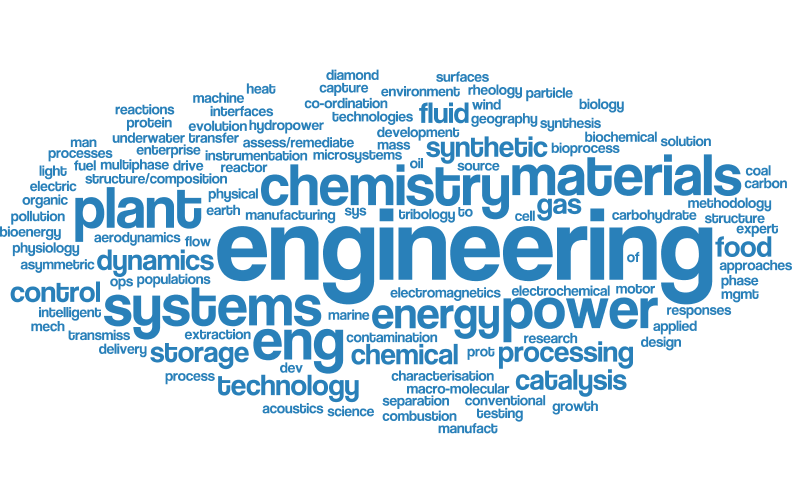
\includegraphics[width=13cm]{word-clouds/number/c3}
    \caption[Topics clustered within Community 3 in the \textit{Topic-grant} network]{Topics clustered within Community 3 in the \textit{Topic-grant} network. Font size represents the number of grants that each topic appears in.}
    \label{figure:topic_a_current_number_c3}
\end{figure}

\noindent\textbf{Community 4 (Mathematics)} is the smallest community in size (only 10 topics) but also the most well-defined community, as the topics clustered within it have a concrete, shared focus in Mathematics. It consists of research topics including \textit{algebra \& geometry}, \textit{mathematical physics} and \textit{continuum mechanics}. \textit{Algebra \& geometry} and \textit{statistics \& appl. probability} are the topics which appear in the highest number of grants, 131 and 120, respectively. In terms of value, the latter is valued higher than the former, \pounds200M compared to \pounds69M. Figure \ref{figure:topic_a_current_number_c4} presents a word cloud representation of Community 4.

\begin{figure}[!htbp]
    \centering
    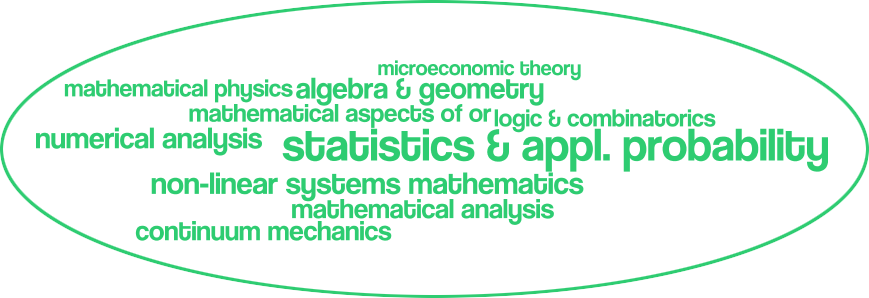
\includegraphics[width=13cm]{word-clouds/number/c4}
    \caption[Topics clustered within Community 4 in the \textit{Topic-grant} network]{Topics clustered within Community 4 in the \textit{Topic-grant} network. Font size represents the number of grants that each topic appears in.}
    \label{figure:topic_a_current_number_c4}
\end{figure}

\noindent\textbf{Community 5 (Environment)} represents a coherent clustering of topics including \textit{energy efficiency}, \textit{geohazards}, \textit{environment \& health} and \textit{urban \& land management}. This community represents topics from different fields which appear in grants that share an aim in tackling an environment-related problem such as climate change or global warming. The most popular topic in terms of number of grants is \textit{energy efficiency}, with 100 grants valued at \pounds150M. Figure \ref{figure:topic_a_current_number_c5} presents a word cloud representation of Community 5.

\begin{figure}[!htbp]
    \centering
    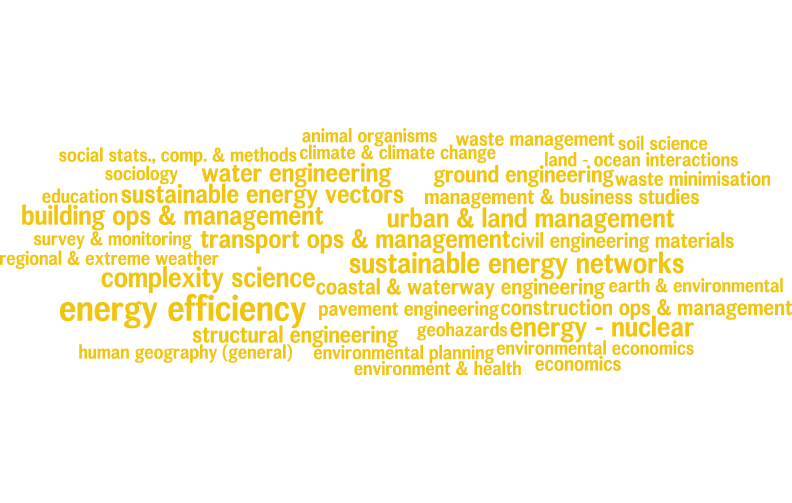
\includegraphics[width=13cm]{word-clouds/number/c5}
    \caption[Topics clustered within Community 5 in the \textit{Topic-grant} network]{Topics clustered within Community 5 in the \textit{Topic-grant} network. Font size represents the number of grants that each topic appears in.}
    \label{figure:topic_a_current_number_c5}
\end{figure}

\noindent\textbf{Community 6 (Physics, Electricity)} is the last identified community and another community which consists of a rational clustering of topics surrounding the fields of \textit{physics} and \textit{electricity}. Topics include \textit{solar technology}, \textit{biophysics} and \textit{electronic devices \& subsys.}. \textit{Condensed Matter Physics} is the topic that appears in in the highest number of grants, 82, worth \pounds97M. Figure \ref{figure:topic_a_current_number_c6} presents a word cloud representation of Community 6.

\begin{figure}[!htbp]
    \centering
    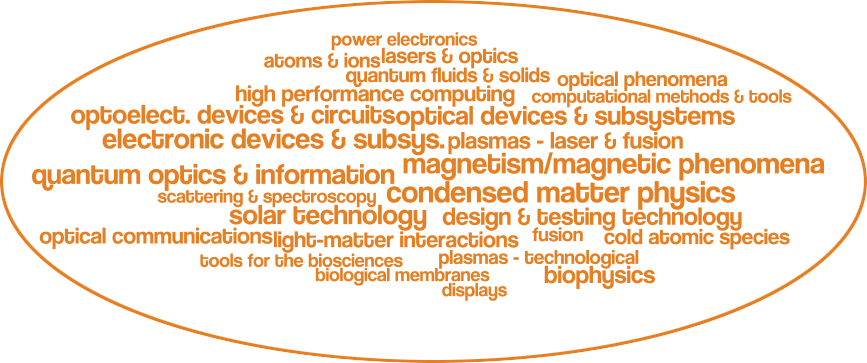
\includegraphics[width=14cm]{word-clouds/number/c6}
    \caption[Topics clustered within Community 6 in the \textit{Topic-grant} network]{Topics clustered within Community 6 in the \textit{Topic-grant} network. Font size represents the number of grants that each topic appears in.}
    \label{figure:topic_a_current_number_c6}
\end{figure}

\noindent Click \href{https://raw.githubusercontent.com/SergiuTripon/msc-thesis-na-epsrc/master/wiki/word-clouds/png/number/communities/modified/full.png?token=AJsbI8Ehc-UcfUTnOVKrCSgHqfUe3IoPks5X27kGwA\%3D\%3D}{\textcolor{blue}{\textbf{here}}} to view a full, high-resolution word cloud representation.

\clearpage

\subsubsection{Visualisation of community structure}

A visualisation of the community structure discovered in the current \textit{Topic-grant} network by the optimal solution identified, presented in Fig. \ref{figure:topic_a_current_cs}, was produced using iGraph. It features nodes in 6 different colours depending on which community they are clustered in. Edges between the nodes in each community are grey, while edges between nodes from different communities are excluded altogether. The size of the node circle represents the number of grants node attribute. The width of the edge line represents the number of grants edge attribute. The topics with the highest number of grants are identified by a darker shade of the colour assigned to their community.

\begin{figure}[htpb]
    \centering
    \fbox{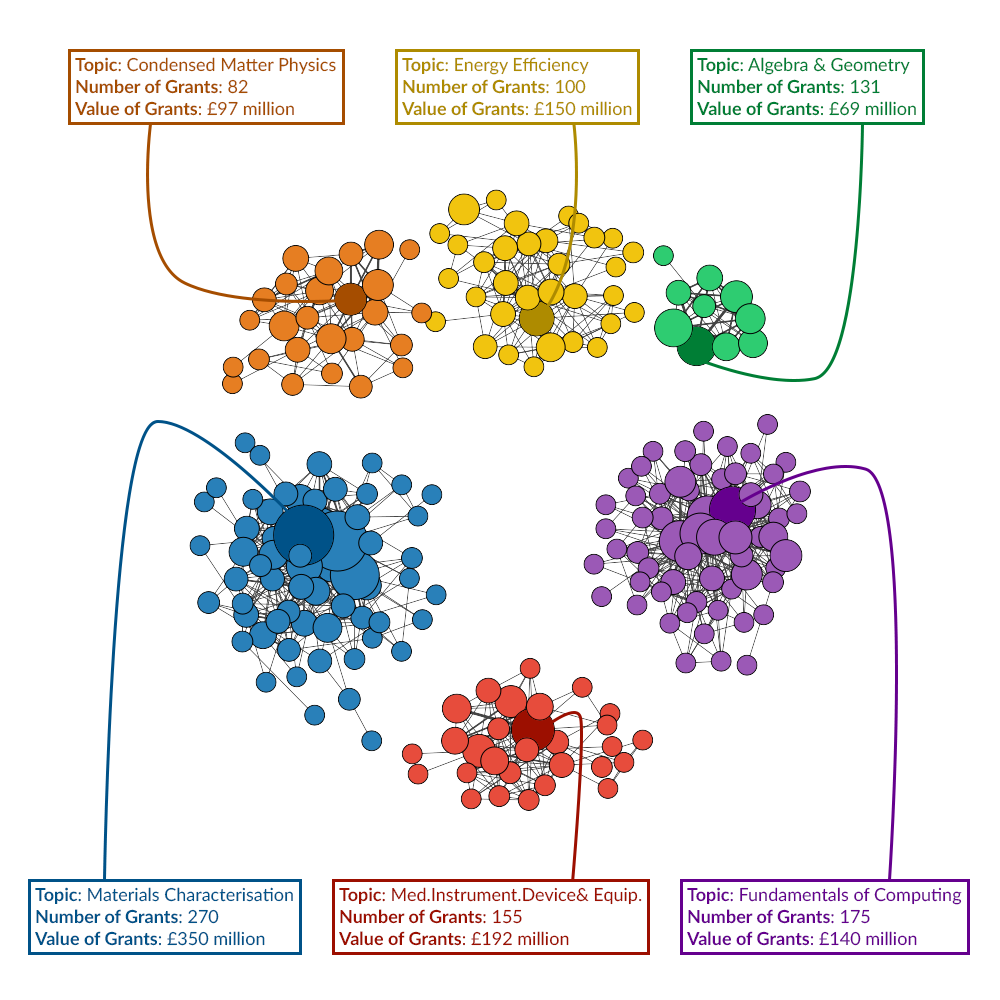
\includegraphics[width=13cm]{communities/topic_a_cs}}
    \caption[Visualisation of the community structure within the \textit{Topic-grant} network constructed using the current (2010 to 2016) data set.]{Visualisation of the community structure within the \textit{Topic-grant} network constructed using the current (2010 to 2016) data set. The topics with the highest number of grants are identified by a darker shade of the colour.}
    \label{figure:topic_a_current_cs}
\end{figure}

\subsection{Evaluation}

A strong network clustering means that a node pair within the same cluster will have a higher similarity compared to a node pair consisting of nodes from two different clusters. The purpose of the evaluation phase is to determine whether in reality this is also true.

First and foremost, the origin and destination nodes of each edge in the \textit{Topic-grant} network were identified. This forms a pair of nodes as follows: (origin node, destination node). Certain edges link nodes that are in the same cluster, while others link nodes that are in different clusters. Therefore, some node pairs represent nodes from the same cluster, while others represent nodes from different clusters. Subsequently, the Dice and Jaccard similarity between each node pair was calculated. Finally, in order to obtain an overall perspective of the similarity of nodes within and between clusters, the average Dice and Jaccard similarity was calculated. 

Indeed, the results show that for both the current and historical Topic-grant networks, nodes within the same cluster have a higher similarity than nodes from different clusters. Table \ref{table:topic_a_evaluation} presents the results of the evaluation phase carried out on the Topic-grant network constructed using both the historical (1990 to 2010) and current (2010 to 2016) data sets.

\begin{table}[htbp]
\centering
\caption[Dice and Jaccard similarity coefficients of node pairs within and between clusters in the Topic-grant constructed using both the historical (1990 to 2010) and current (2010 to 2016) data sets.]{Dice and Jaccard similarity coefficients of node pairs within and between clusters in the Topic-grant network constructed using both the historical (1990 to 2010) and current (2010 to 2016) data sets. Each node pair represents an edge which links two nodes from the same cluster or two different clusters. \textbf{IN} stands for within communities, while \textbf{OUT} means between communities.}
\label{table:topic_a_evaluation}
\begin{tabular}{r|rrr}
{} & \textbf{1990-2000} & \textbf{2000-2010} & \textbf{2010-2016}\\
\hline\\
Node pairs IN                  & {437}   & {1940}  & {1122}\\
Node pairs OUT                 & {311}   & {1652}  & {886}\\
Average Dice similarity IN     & {0.465} & {0.510} & {0.428}\\
Average Dice similarity OUT    & {0.346} & {0.433} & {0.354}\\
Difference between IN and OUT  & {0.119} & {0.077} & {0.074}\\
Average Jaccard similarity IN  & {0.316} & {0.356} & {0.286}\\
Average Jaccard similarity OUT & {0.217} & {0.283} & {0.220}\\
Difference between IN and OUT  & {0.099} & {0.073} & {0.066}\\
\end{tabular}
\end{table}

\clearpage

\subsection{Discussion}

The \textit{Topic-grant} network was constructed using both the historical (1990 to 2010) and current (2010 to 2016) data sets. This means a comparative analysis can be conducted comparing the data sets in terms of research trend and funding, and clustering.

\subsubsection{Comparison to historical data}

Over the years, the research trend led to new topics being defined, while others were discontinued. For example, \textit{bionanoscience}, \textit{escience} and \textit{language acquisition} are topics which existed \textit{from 2000 to 2010} but do not exist currently. In contrast, \textit{animal organisms}, \textit{political geography} and \textit{ageing: chemistry/biochemistry} are some of the current topics that were defined after 2010.

Similarly, the funding trend also evolved as more recent grants saw a significant increase in the funding support provided. Currently, there are 3,072 grants within communities with a total value of \pounds3.5B. Between 2000 and 2010, researchers worked on 16,617 grants, valued at \pounds4.9B. These figures indicate a significant difference in the number of grants. However, this is justified, as the two time periods compared are not equal, as the former covers 6 years of grants, while the latter covers 10 years. More importantly, the difference in value is not considerable, which shows the progress of research funding over the years, as current grants receive significantly more funding than they would have 10 years ago.

Furthermore, this is also supported by the number and value of grants completed between 1990 and 2000. Researchers worked on a slightly less number of grants than between 2000 and 2010, but they also received significantly less funding, \pounds1.7B. Tables \ref{table:topic_a_past1_numbers} and \ref{table:topic_a_past2_numbers} present the number of nodes representing topics, the number and value of grants and the predominant words within each community in the \textit{Topic-grant} network constructed using the historical (2000 to 2010) data set and historical (1990 to 2000) data set, respectively.

\clearpage

\begin{table}[!htbp]
\centering
\caption[Number of nodes and grants, value of grants and the predominant words of each community identified in the \textit{Topic-grant} network constructed using the historical (2000 to 2010) data set]{Number of nodes and grants, value of grants and the predominant words based on word frequency of each community identified in the \textit{Topic-grant} network constructed using the historical (2000 to 2010) data set. The number of grants includes duplicate grants, as a grant can be part of more than one community. Subsequently, the value of grants also includes the duplicate grants. However, the last column represents the number and value of unique grants in communities within the historical \textit{Topic-grant} network.}
\label{table:topic_a_past1_numbers}
\begin{tabular}{r|>{\raggedleft\arraybackslash}p{1.6cm}>{\raggedleft\arraybackslash}p{1.6cm}>{\raggedleft\arraybackslash}p{1.6cm}>{\raggedleft\arraybackslash}p{6.3cm}}
{} & \textbf{Number (topics)} & \textbf{Number (grants)} & \textbf{Value (grants)} & \textbf{Predominant words based on word frequency}\\
\hline\\
\textbf{C1}  & {67}  & {8682}  & {\pounds2.6B} & {chemistry, biology, science}\\
\textbf{C2}  & {43}  & {5167}  & {\pounds1.3B} & {engineering, mathematical}\\
\textbf{C3}  & {25}  & {1394}  & {\pounds699M} & {energy, power}\\
\textbf{C4}  & {2}   & {1}     & {\pounds1M}   & {science}\\
\textbf{C5}  & {71}  & {4099}  & {\pounds1.3B} & {design, arts, digital}\\
\hline\\
\textbf{All} & {208} & {16617} & {\pounds4.9B} & {engineering, biology, design}\\
\end{tabular}
\end{table}

In terms of clustering, the historical communities identified within the \textit{Topic-grant} network hold slight differences when compared to the current communities. First and foremost, the community detection algorithm identified 5 communities in both historical (1990 to 2000, 2000 to 2016) networks. This decrease may signify the result of the contrast in the number of topics and the actual topics between the current and historical networks. Moreover, the most well-defined, Community 4 (Mathematics) identified in the current \textit{Topic-grant} network, is not as well-defined anymore in the historical network, as it is part of a larger community in Community 2 (Engineering, Mathematics ). This symbolises the current increase in the number of grants that are focused on \textit{mathematics} only, rather than a combined effort including other topics such as \textit{engineering}. Furthermore, between 2000 and 2010, only one grant was classified simultaneously by \textit{soil science} and \textit{crop science}. In the current (2010 to 2016) data set, \textit{crop science} is not present anymore. Perhaps, its removal could be justified by the similarity between the two topics, deeming one of them as unnecessary. This also indicates a potential reason why the two topics did not form a community in the current \textit{Topic-grant} network.

\begin{table}[!htbp]
\centering
\caption[Number of nodes and grants, value of grants and the predominant words of each community identified in the \textit{Topic-grant} network constructed using the historical (1990 to 2000) data set]{Number of nodes and grants, value of grants and the predominant words based on word frequency of each community identified in the \textit{Topic-grant} network constructed using the historical (1990 to 2000) data set. The number of grants includes duplicate grants, as a grant can be part of more than one community. Subsequently, the value of grants also includes the duplicate grants. However, the last column represents the number and value of unique grants in communities within the historical \textit{Topic-grant network}.}
\label{table:topic_a_past2_numbers}
\begin{tabular}{r|>{\raggedleft\arraybackslash}p{1.6cm}>{\raggedleft\arraybackslash}p{1.6cm}>{\raggedleft\arraybackslash}p{1.6cm}>{\raggedleft\arraybackslash}p{6.3cm}}
{} & \textbf{Number (topics)} & \textbf{Number (grants)} & \textbf{Value (grants)} & \textbf{Predominant words based on word frequency}\\
\hline\\
\textbf{C1}  & {28}  & {2015}  & {\pounds246M} & {engineering, energy, management}\\
\textbf{C2}  & {25}  & {3995}  & {\pounds661M} & {optical, devices, materials}\\
\textbf{C3}  & {17}  & {1328}  & {\pounds88M}  & {mathematical, analysis}\\
\textbf{C4}  & {39}  & {3455}  & {\pounds496M} & {engineering, ict, design}\\
\textbf{C5}  & {27}  & {2567}  & {\pounds385M} & {chemistry, catalysis, energy}\\
\hline\\
\textbf{All} & {136} & {12791} & {\pounds1.7B} & {engineering, chemistry, systems}\\
\end{tabular}
\end{table}

\subsubsection{Motivation for the Topic-researcher network}

The \textit{Topic-researcher} network represents an alternative and another way of interpreting the topic data to construct a network. An alternative represents a different perspective on the data. The \textit{Topic-grant} network is one way of analysing topics, from the point of view of grants. The \textit{Topic-researcher} network is a second way of analysing topics, from the point of view of researchers. Grant records and researcher records are significantly different, and one may provide different or better results than the other. Furthermore, having a different way of analysing the data means that a comparative analysis of the results can be carried out. Therefore, both networks are considered important due to the different and valuable insights that can be translated from the data.

\clearpage

\section{Clustering of Topic-researcher network}

The process of clustering the \textit{Topic-researcher} network involves a number of different stages including carrying out experiments, producing results, evaluating results as well as conducting comparative analysis.

\subsection{Experiment}

In order to ensure a consistent comparative analysis between the two Topic networks, the optimal solution identified as a result of the experiment on the \textit{Topic-grant} network, is also considered the optimal solution for the \textit{Topic-researcher} network. However, the experiment was still carried out and the results are presented in Tables 1.31-1.33, part of the Supplementary material.

\subsection{Results}

The application of the optimal solution identified on the \textit{Topic-researcher} network resulted in the identification of 4 different communities of topics, 2 less than within the \textit{Topic-grant} network. Note that the \textit{Topic-researcher} network was constructed using the current (2010 to 2016) data set only, as researcher records within EPSRC only provide the current topics of a researcher. Table \ref{table:topic_b_current_numbers} presents the number of nodes representing topics and the predominant words within each community discovered in the \textit{Topic-researcher} network. The complete clustering of the \textit{Topic-researcher} network is presented in Table \ref{table:topic_b_current_clusters_appendix}, part of Appendix \ref{appendix:epsrc_grant_data}.

\begin{table}[!htbp]
\centering
\caption[Number of nodes and the predominant words of each community identified in the \textit{Topic-researcher} network constructed using the current (2010 to 2016) data set]{Number of nodes and the predominant words based on word frequency of each community identified within the \textit{Topic-researcher} network constructed using the current (2010 to 2016) data set.}
\label{table:topic_b_current_numbers}
\begin{tabular}{r|>{\raggedleft\arraybackslash}p{1.6cm}>{\raggedleft\arraybackslash}p{6.5cm}}
{} & \textbf{Number (topics)} & \textbf{Predominant words based on frequency of words}\\
\hline\\
\textbf{C1}  & {39}  & {engineering, management}\\
\textbf{C2}  & {62}  & {psychology, design}\\
\textbf{C3}  & {15}  & {mathematical, analysis}\\
\textbf{C4}  & {109} & {engineering, chemistry}\\
\hline\\
\textbf{All} & {225} & {engineering, management, science}\\
\end{tabular}
\end{table}

\subsubsection{Visualisation of community structure}

Similarly to the \textit{Topic-grant} network, a visualisation of the community structure discovered in the current \textit{Topic-researcher} network was produced and is presented in Fig. \ref{figure:topic_b_current_cs}.

\begin{figure}[htpb]
    \centering
    \fbox{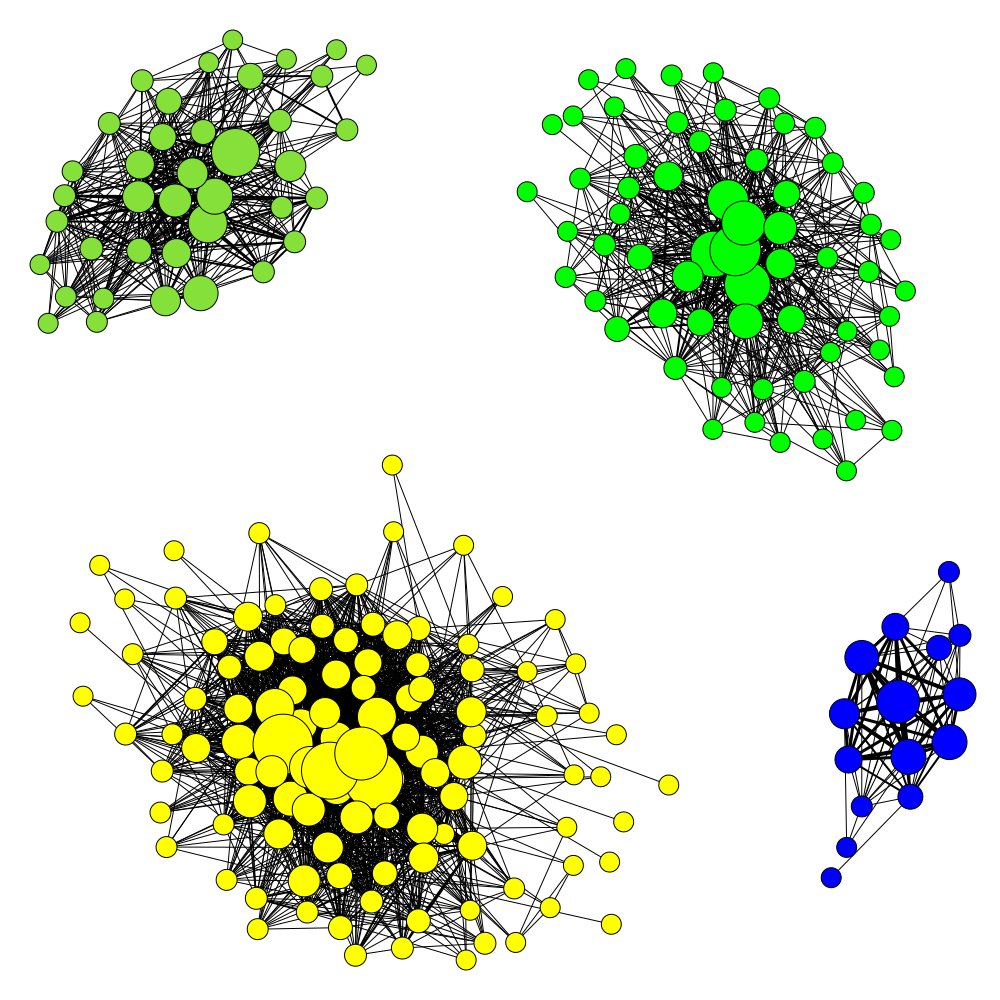
\includegraphics[width=13.8cm]{communities/topic_b_cs}}
    \caption[Visualisation of the community structure within the Topic-researcher network constructed using the current (2010 to 2016) data set.]{Visualisation of the community structure within the Topic-researcher network constructed using the current (2010 to 2016) data set.}
    \label{figure:topic_b_current_cs}
\end{figure}

\subsection{Evaluation}

Similarly to the \textit{Topic-grant} network, the \textit{Topic-researcher} network also underwent the evaluation phase and the results show that for both the current and historical \textit{Topic-researcher} networks, nodes within the same cluster have a higher similarity than nodes from different clusters. Table \ref{table:topic_b_evaluation} presents the results of the evaluation phase carried out on the \textit{Topic-researcher} network constructed using the current (2010 to 2016) data set.

\begin{table}[htpb]
\centering
\caption[Dice and Jaccard similarity coefficients of node pairs within and between clusters in the \textit{Topic-researcher} constructed using the current (2010 to 2016) data set.]{Dice and Jaccard similarity coefficients of node pairs within and between clusters in the \textit{Topic-researcher} network constructed using the current (2010 to 2016) data set. Each node pair represents an edge which links two nodes from the same cluster or two different clusters. \textbf{IN} stands for within communities, while \textbf{OUT} means between communities.}
\label{table:topic_b_evaluation}
\begin{tabular}{r|r}
{} & \textbf{2010-2016}\\
\hline\\
Node pairs IN                  & {2921}\\
Node pairs OUT                 & {2271}\\
Average Dice similarity IN     & {0.543}\\
Average Dice similarity OUT    & {0.517}\\
Difference between IN and OUT  & {0.026}\\
Average Jaccard similarity IN  & {0.393}\\
Average Jaccard similarity OUT & {0.359}\\
Difference between IN and OUT  & {0.034}\\
\end{tabular}
\end{table}

\subsection{Discussion}

The \textit{Topic-grant} and \textit{Topic-researcher} networks represent two interpretations of the topic data. This means a comparative analysis can be conducted comparing the two networks in terms of clustering.

\subsubsection{Comparison to Topic-grant network}

There are obvious differences between the clustering produced using the \textit{Topic-grant} network and \textit{Topic-researcher} network. Firstly, the number of communities identified differs, as using the former 6 communities were identified, compared to 4 when using the latter. This results in an imbalance in community size, with one of the communities (Community 4) identified in the \textit{Topic-researcher} network consisting of 109 topics. A large community is also a broad community, which means that is less specific and lacks the capability to represent one or more clear research areas. It also causes other communities to be significantly smaller in size.

\clearpage

Furthermore, the \textit{Mathematics} community (Community 4) identified using the \textit{Topic-grant} network is larger in size and its previously well-defined structure is "harmed" by the irrational addition of topics such as \textit{genomics} when identified  using the \textit{Topic-researcher} network. Moreover, the clustering produced using the \textit{Topic-researcher} network also failed to identify the \textit{Biology} community (Community 1) which was successfully identified using the \textit{Topic-grant} network. That being said, there are also similarities between the communities identified using the two networks, as the \textit{Engineering} and \textit{Chemistry} communities appear in the community structure of both networks.

In conclusion, it is concluded that the clustering produced using the \textit{Topic-grant} network is more coherent and balanced than the one produced using the \textit{Topic-researcher} network.